%% ---------------------------------------------------------------------------
%% intro.tex
%%
%% Introduction
%%
%% $Id: intro.tex 1477 2010-07-28 21:34:43Z palvarado $
%% ---------------------------------------------------------------------------

\chapter{Introduction}
\label{chp:intro}

\section{Video artifacts in live video streaming}
\label{sec:intro_artifacts}

Modern day streaming services are fundamental instruments in modern industries, institutions, and every day life. For instance, live video conferencing and streaming services became the principal mediums of communication for a large sector of national and global society during the recent COVID-19 pandemic.

The recent COVID-19 pandemic exemplified the role of video conferencing and live streaming services in today's society. Current advances in network speed and digital technology have enabled these services to become commonplace in professional, academic, and recreational contexts. Therefore, there has been increased interest in ensuring a high quality of experience (QoE) for these services.

One of the main issues affecting the QoE of video conferencing and live streaming services is video artifacts, as mentioned in \cite{Vranjes2018, Korhonen2018}. In \cite{Greengrass2009}, video artifacts, or simply artifacts, are defined as distortions in the images displayed to the user with respect to the original captured images. According to \cite{Vranjes2018}, artifacts are primarily caused by errors or loss of data in the transmission of the video over the network, or by losses caused during video compression. Figure \ref{fig:1.1} compares two versions of the same image. Figure \ref{fig:1.1.a} contains no video artifacts and Figure \ref{fig:1.1.b} contains video artifacts due to packet loss.

\begin{figure} [!h]
  \centering
  
  \begin{subfigure}[t]{0.49\textwidth}
    \centering
    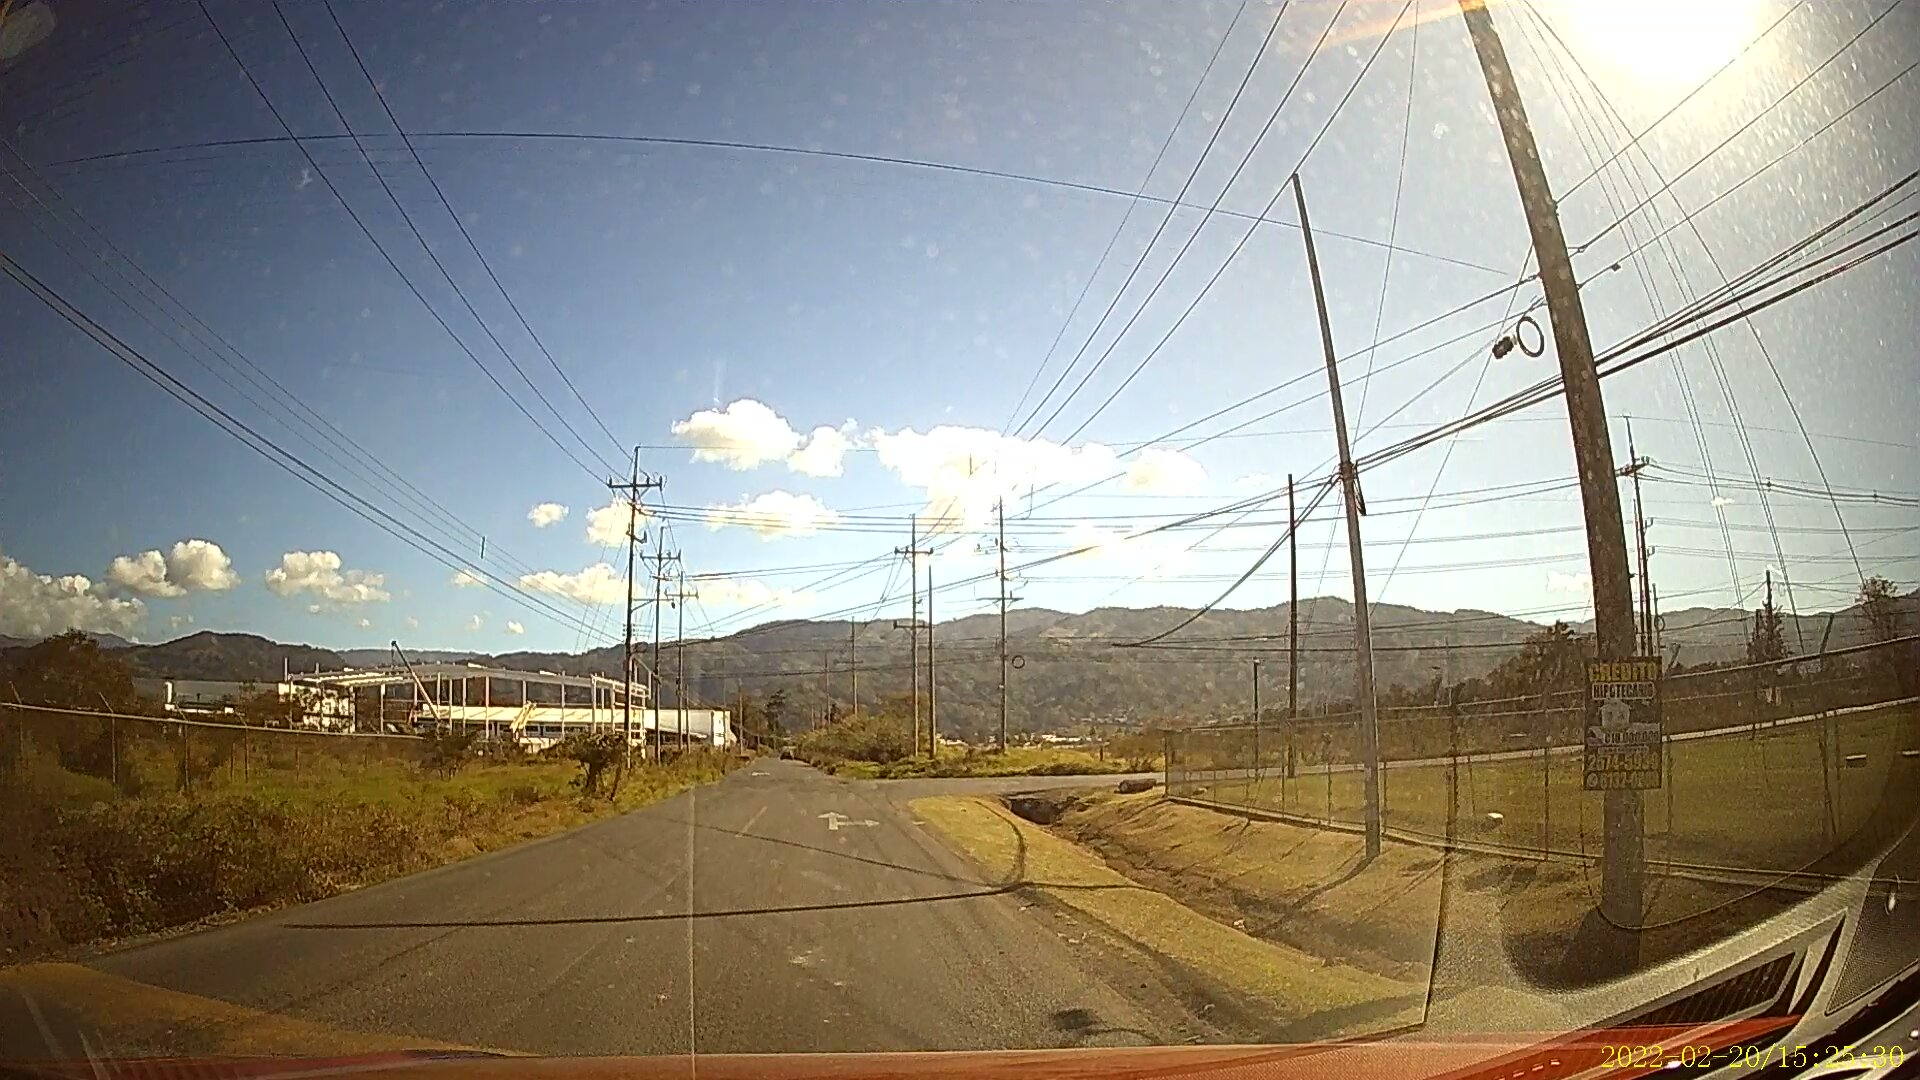
\includegraphics[width=\textwidth]{imgs_27}
    \caption{Frame with no video artifacts}
    \label{fig:1.1.a}
  \end{subfigure}
  \hfill
  \begin{subfigure}[t]{0.49\textwidth}
    \centering
    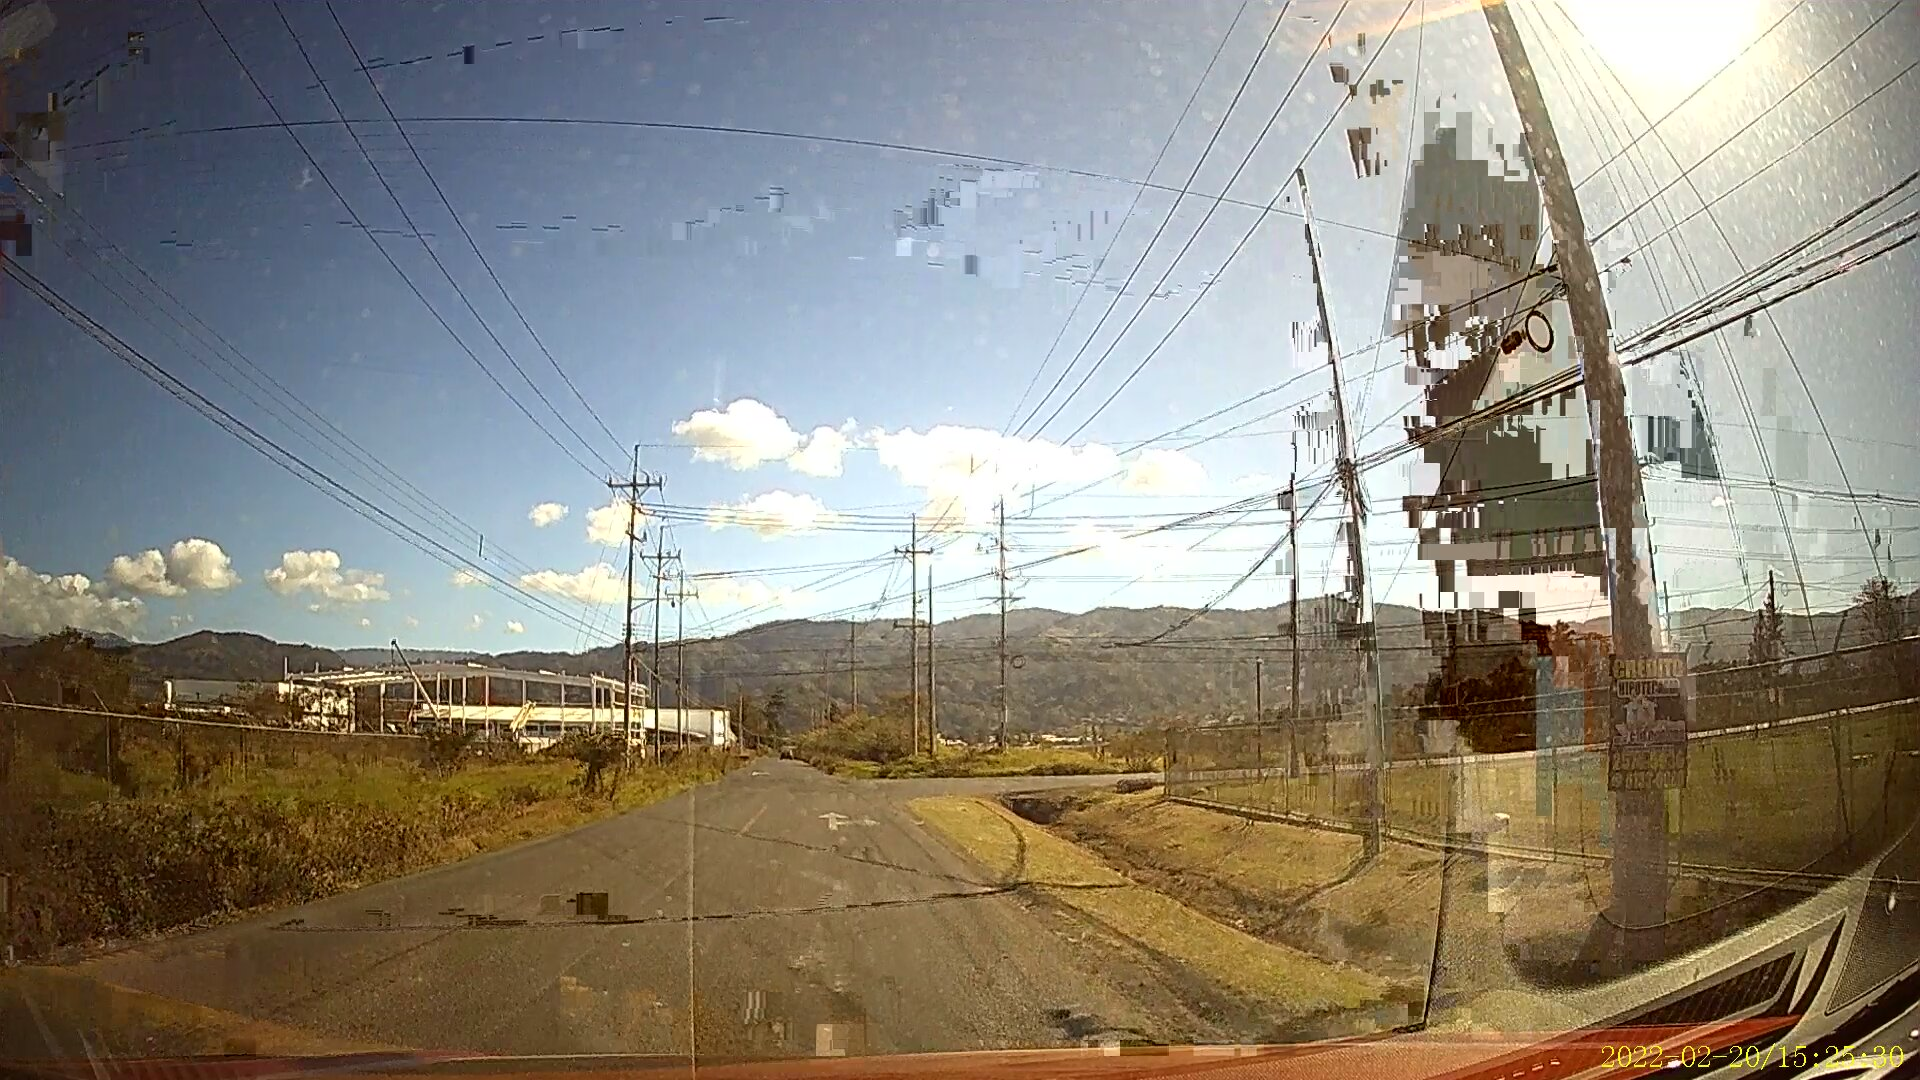
\includegraphics[width=\textwidth]{imgs_with_loss_27}
    \caption{Frame with video artifacts due to packet loss}
    \label{fig:1.1.b}
  \end{subfigure}
  
  \caption{Comparison between a video frame with no artifacts and a video frame with artifacts caused by random h264 packet loss.}
  \label{fig:1.1}

\end{figure}

There are methods to solve transmission errors in the transport layer or even in the video syntax layer, as mentioned in \cite{Sanyal2021}. In these cases, information is available on how the video packets are encoded, which simplifies the task of error detection and correction. When the user only has the decoded and decompressed information, it is necessary to use methods for artifact detection and correction that only have the pure video information, such as those of \cite{Vranjes2018, Sanyal2021,Goodall2019}. These methods are referred to as ``reference-free methods''.

Video artifacts result in loss of information from the original video. In video conferencing and live streaming applications, it is not possible to recover the lost data without affecting the user's QoE. In order to correct video artifacts, reference-free methods must infer the lost data. The process of restoring unknown areas of an image is called ``video restoration'' \cite{Li2022, Zhou2021}. Video restoration, or simply restoration, is commonly used to remove the presence of objects in a video or image, but can be used to reconstruct areas of an image affected by video artifacts, as is done in ``video restoration'' \cite{Dong2023, Brenes2022}.

Modern restoration algorithms use machine learning models. The restorers of \cite{Li2022, Zhou2021, Liu2021} use ``transformers''. Transformers are machine learning models with outstanding results for signal reconstruction tasks, but they are expensive in both time and processing power. In order to optimize the performance of these models, the use of hardware accelerators is required, the most common being the GPU.

Restoration models such as \cite{Li2022} require binary masks to identify the areas to be reconstructed. For this reason, the location of video artifacts must be detected and binary masks must be generated and then used in the image reconstruction stage.

Classifications of different types of artifacts by packet loss exist \cite{Greengrass2009, Glavota2016}. These studies describe the statistical properties of video artifacts. For example, certain video artifacts tend to have high-contrast vertical and horizontal edges that can be detected by high-pass filters. In the MPEG and H.26x video compression standards, the pixels of an image are grouped into ``macroblocks'', which are groups of $16 \times 16$ pixels in the image. Losses of packets containing macroblock information result in artifacts with well-defined edges \cite{Vranjes2019, Glavota2018}.

Methods for video artifact detection from \cite{Vranjes2018, Glavota2018} focus on filtering algorithms that do not involve machine learning. These methods can reach processing more than 30 video frames per second counting only CPU resources, but they oversimplify the characteristics of video artifacts and fail to achieve high detection rates. There are also artifact detection methods using neural networks, such as those of \cite{Goodall2019, Rajasekar2020}. These methods generalize better than filtering algorithms, but are more resource-heavy and require accelerators, such as GPUs, to achieve speeds comparable to filtering algorithms.

During 2022, SIPLab developed the dispTEC2-2022 project in conjunction with the company RidgeRun for the restoration of video with packet loss artifacts. The project was developed on Nvidia's Jetson TX2. This system has a 256 CUDA-core GPU, 4 ARM CPUs and 2 Denver CPUs. The development of the image reconstruction stage of dispTEC2-2022 is detailed in \cite{Brenes2022}. This model uses the GPU in its entirety. Brenes' reconstruction model requires binary masks to locate artifacts in the input images and the project in general still lacks an artifact detection method.

\section{The 2022 dispTEC project}
\label{sec:intro_disptec}

\section{Video Artifact Detection}
\label{sec:intro_problem}

One objective of video artifact correction in video conferencing and live streaming applications is to ensure high QoE for the end user. In addition, video artifact correction has an artifact detection stage and an artifact restoration stage. The trade-off between the computational cost of these processes and the QoE requirements for the end user complicates the development of a video artifact correction system.

Quality criteria must be established to determine if the artifact correction process performs adequately. The quality perceived by the end user depends on at least two criteria: the speed of the final video and the image quality in the final video.

To determine an appropriate video speed criterion, Zoom is considered as an example of a video conferencing application. According to \cite{ZoomSupport}, Zoom recommends using the application at a resolution of $1280 \times 720$ pixels and at 30 frames per second. Under this recommendation, an obstacle facing artifact detection and restoration processing is to manage to operate on frames of $1280 \times 720$ pixels at a rate of 30 frames per second. In terms of processing time, each frame must be processed in about 33 ms. For the purposes of this paper, this processing speed is referred to as ``real time''.

For each frame, it is necessary to detect the locations of video artifacts and then perform the restoration process. For the total processing to happen in real time, both the detection stage and the restoration stage must take even less time than 33 ms per frame.

Restoration processing, which relies on the use of neural networks, requires the use of hardware acceleration to achieve real-time processing. Therefore, consideration must be given to the resources available on the equipment on which video artifact correction is performed.

If video artifact correction occurs on the same device, the detection process must share resources with the restoration process. Considering that the restoration process requires an accelerator, it must be considered that the resources available for the detection process are limited.

The quality of the final video depends on both the effectiveness of the detection process and the capability of the restoration process. The effectiveness of the detection process can be measured through the metrics of accuracy and completeness. Using the definitions of \cite{ScikitLearn}, accuracy is the ratio of the number of correct detections to the number of total detections. Completeness is the ratio between the number of correct detections and the number of detections that should ideally be obtained. To ensure a high quality of artifact detection, the accuracy and completeness criteria of the detection method must be considered.

The algorithmic complexity of the detection method directly affects the processing power required to perform the detection. The resources available for detection affect both the speed and the processing power available for detection. Therefore, the trade-off between available resources, speed of detection, and quality of detection must be considered.

The work of \cite{Brenes2022} performs the image restoration process and runs on an Nvidia Jetson TX2. It uses the entire GPU to run. This job lacks an artifact detector to identify the image areas to be restored.

No existe un método de detección de artefactos de video para ser utilizado en restauración de video en tiempo real que considere el compromiso entre la administración de recursos disponibles en el equipo a emplear, la velocidad a tiempo real que se desea alcanzar y la calidad del método de detección.

There is no video artifact detection method for use in real-time video restoration that considers the trade-off between the management of available resources in the equipment to be used, the desired real-time speed and the quality of the detection method.

\section{Random Forest Detector}
\label{sec:intro_detector}

The most appropriate solution to the video artifact detection problem is the implementation of a Random Decision Forest. Forests have advantages over the other possible solutions given the speed, resource and quality constraints that must be considered. Filtering algorithms are resource efficient and fast, but they are limited in their ability to generalize to a wide variety of artifacts, so they do not have the best detection quality. Neural networks are powerful algorithms and result in the best detection results, but they consume more resources than are available for artifact detection. If neural networks are run with limited resources, the processing time increases significantly. Random Decision Forests are capable of generalizing detection tasks with \cite{Keskin2012} images, as well as being efficient in resource uses and speed. For this reason Random Decision Forests are the most appropriate solution for the problem to be solved.

\section{Project objectives and document structure}
\label{sec:intro_objectives}

\section{Introduction Outline}
\label{sec:intro_outline}

\begin{enumerate}
  \item Hook: Convince reader that real time video transmission is important and interesting. The idea being that these are used everywhere nowdays.
  \item Then make the argument that because of this, it is important to assure a good QoS.
  \item Then talk about possible challenges to QoS. Here might be the place to mention macroblock errors. Consider justifying that in some contexts, only the raw stream is obtained.
  \item Then talk about possible solutions to problem.
  \item Perhaps use a few paragraphs to detail how correction is broken down into detection, then repainting.
\end{enumerate}

\subsection{Antecedentes}

\begin{enumerate}
  \item Introduce dispTEC2 - What is it? What was it trying to accomplish
  \item Here might be a good place for the complete block diagram
  \item Explain the challenges in designing for the TX2 and how dispTEC2 decided to face them.
  \item Explain the work done in inpainting and mention Greivin's results
  \item Explain the work done in decoding and give some results
  \item Explain challenges in decoder
\end{enumerate}

\subsection{Planteamiento del problema}

\begin{enumerate}
  \item This part may link with with previous section, continuing off the challenges in the decoder
  \item Perhaps here I can use diagrams to be clear with every challenge
  \item Address resource challenges, why can detection only use CPU?
  \item Address performance challenges, why must it run at 30 fps?
  \item Address previous work challenges with using PLDA algorithm and such
  \item Finally, sinthetize the problem
\end{enumerate}

\subsection{Propuesta de solución}

\begin{enumerate}
  \item Here introduce a variety of different solutions for this problem
  \item Introduce the advantages and disadvantages of each one
  \item Perhaps talk about using detection algorithms
  \item Then talk about using neural network
  \item Then talk about other machine learning alternatives
  \item Finally, talk about how RDFs are the best solution for my specific situation
  \item Use block diagram to show design
  \item 
\end{enumerate}

\subsection{Objetivos y estructura del documento}

\begin{enumerate}
  \item Here I can almost use the same objectives from project proposal
\end{enumerate}

